% move all configuration stuff into includes file so we can focus on the content
\documentclass[aspectratio=169,hyperref={pdfpagelabels=false,colorlinks=true,linkcolor=white,urlcolor=gtgold},t]{beamer}

%%%%%%%%%%%%%%%%%%%%%%%%%%%%%%%%%%%%%%%%%%%%%%%%%%%%%%%%%%%%%%%%%%%%%%%%%%%%%%%%%%
%%%%%%%%%%%%%%%%%%%%%%%%%%%%%%%%%%%%%%%%%%%%%%%%%%%%%%%%%%%%%%%%%%%%%%%%%%%%%%%%%%
% packages
\usepackage{pict2e}
\usepackage{epic}
\usepackage{amsmath,amsfonts,amssymb}
\usepackage{units}
\usepackage{fancybox}
\usepackage[absolute,overlay]{textpos} 
%\usepackage{media9} % avi2flv: "C:\Program Files\ffmpeg\bin\ffmpeg.exe" -i TuneFreqFilterbank.avi -b 600k -s 441x324 -r 15 -acodec copy TuneFreqFilterbank.flv
\usepackage{animate}
\usepackage{gensymb}
\usepackage{multirow}
\usepackage{silence}
\usepackage{tikz}
\usepackage[backend=bibtex,style=ieee]{biblatex}
\AtEveryCitekey{\iffootnote{\tiny}{}}
\addbibresource{include/references}



% fontsize
\let\Tiny=\tiny

%%%%%%%%%%%%%%%%%%%%%%%%%%%%%%%%%%%%%%%%%%%%%%%%%%%%%%%%%%%%%%%%%%%%%%%%%%%%%%%%%%
%%%%%%%%%%%%%%%%%%%%%%%%%%%%%%%%%%%%%%%%%%%%%%%%%%%%%%%%%%%%%%%%%%%%%%%%%%%%%%%%%%
% warnings
\pdfsuppresswarningpagegroup=1
\WarningFilter{biblatex}{Patching footnotes failed}
\WarningFilter{latexfont}{Font shape}
\WarningFilter{latexfont}{Some font shapes}
\WarningFilter{gensymb}{Not defining}


%%%%%%%%%%%%%%%%%%%%%%%%%%%%%%%%%%%%%%%%%%%%%%%%%%%%%%%%%%%%%%%%%%%%%%%%%%%%%%%%%%
%%%%%%%%%%%%%%%%%%%%%%%%%%%%%%%%%%%%%%%%%%%%%%%%%%%%%%%%%%%%%%%%%%%%%%%%%%%%%%%%%%
% theme & layout
\usetheme{Frankfurt}
\useinnertheme{rectangles}


%%%%%%%%%%%%%%%%%%%%%%%%%%%%%%%%%%%%%%%%%%%%%%%%%%%%%%%%%%%%%%%%%%%%%%%%%%%%%%%%%%
\setbeamertemplate{frametitle}[default][colsep=-4bp,rounded=false,shadow=false]
\setbeamertemplate{frametitle}
{%
    \nointerlineskip%
    \begin{beamercolorbox}[wd=\paperwidth,ht=3.5ex,dp=0.6ex]{frametitle}
        \hspace*{1.3ex}\insertframetitle%
        
        \hspace*{1.3ex}\small\insertframesubtitle%
    \end{beamercolorbox}%
    \begin{textblock*}{100mm}(11.6cm,.57cm)
        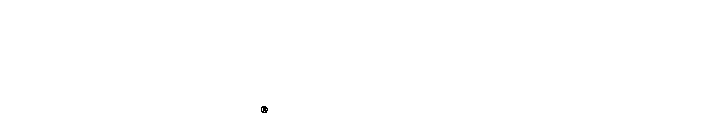
\includegraphics[height=.8cm,keepaspectratio]{graph/Logo_GTCMT_white}
    \end{textblock*}
}


%%%%%%%%%%%%%%%%%%%%%%%%%%%%%%%%%%%%%%%%%%%%%%%%%%%%%%%%%%%%%%%%%%%%%%%%%%%%%%%%%%
\setbeamertemplate{title page}[default][colsep=-4bp,rounded=false,shadow=false]
\setbeamertemplate{title page}
{
    \begin{textblock*}{200mm}(13.5cm,.5cm)
            \href{https://github.com/alexanderlerch/\jobname}{
\includegraphics[height=2cm,keepaspectratio]{graph/qr}}\hspace*{2ex}
    \end{textblock*}
    \vskip-10ex
    \begin{beamercolorbox}[wd=\paperwidth,ht=.7\paperheight,dp=0.6ex]{frametitle} %35ex
        \hspace*{1.8ex}\LARGE\inserttitle%
        
        \vspace*{.5ex}
        
        \hspace*{1.3ex}\small\insertsubtitle%
        
        \vspace*{.5ex}
    \end{beamercolorbox}%
    \nointerlineskip%
    \begin{beamercolorbox}[wd=\paperwidth,ht=.4\paperheight,dp=0.6ex]{page number in head/foot}
        %\vspace*{-.5ex}
        \hspace*{1.7ex}\small\insertauthor%
        
        %\hspace*{1.7ex}\small }%
        
        \vspace*{10ex}
        
        \begin{flushright}
            \href{http://www.gtcmt.gatech.edu}{
\includegraphics[height=.8cm,keepaspectratio]{graph/Logo_GTCMT_black}}\hspace*{2ex}
        \end{flushright}
    \end{beamercolorbox}%
		\addreference{\hspace{32mm}\href{https://github.com/alexanderlerch/2023-FRSM}{github.com/alexanderlerch/\jobname}}
}


%%%%%%%%%%%%%%%%%%%%%%%%%%%%%%%%%%%%%%%%%%%%%%%%%%%%%%%%%%%%%%%%%%%%%%%%%%%%%%%%%%
%\makeatother
\setbeamertemplate{footline}
{
  \leavevmode%
  \hbox{%
  \begin{beamercolorbox}[wd=.5\paperwidth,ht=2.25ex,dp=1ex,left,leftskip=1ex]{page number in head/foot}%
    \insertsubtitle
  \end{beamercolorbox}%
  \begin{beamercolorbox}[wd=.5\paperwidth,ht=2.25ex,dp=1ex,right,rightskip=1ex]{page number in head/foot}%
    \hfill
    \insertframenumber{} / \inserttotalframenumber
  \end{beamercolorbox}}%
  \vskip0pt%
}
%\makeatletter


%%%%%%%%%%%%%%%%%%%%%%%%%%%%%%%%%%%%%%%%%%%%%%%%%%%%%%%%%%%%%%%%%%%%%%%%%%%%%%%%%%
\beamertemplatenavigationsymbolsempty
\setbeamertemplate{navigation symbols}{}
\setbeamertemplate{blocks}[default]%[rounded=false,shadow=false]
\setbeamertemplate{itemize item}[square]
\setbeamertemplate{itemize subitem}[circle]
\setbeamertemplate{itemize subsubitem}[triangle]
\setbeamertemplate{enumerate item}[square]
\setbeamertemplate{enumerate subitem}[circle]
\setbeamertemplate{enumerate subsubitem}[circle]


%%%%%%%%%%%%%%%%%%%%%%%%%%%%%%%%%%%%%%%%%%%%%%%%%%%%%%%%%%%%%%%%%%%%%%%%%%%%%%%%%%
% colors
\setbeamercolor{structure}{fg=darkgray}
\setbeamercovered{transparent} %invisible
\setbeamercolor{bibliography entry author}{fg=black}
\setbeamercolor*{bibliography entry title}{fg=black}
\setbeamercolor*{bibliography entry note}{fg=black}
\setbeamercolor{frametitle}{fg=black}
\setbeamercolor{title}{fg=white}
\setbeamercolor{subtitle}{fg=white}
\setbeamercolor{frametitle}{fg=white}
\setbeamercolor{framesubtitle}{fg=white}
\setbeamercolor{mini frame}{fg=white, bg=black}
\setbeamercolor{section in head/foot}{fg=white, bg=darkgray}
\setbeamercolor{page number in head/foot}{fg=black, bg=gtgold}
\setbeamercolor{item projected}{fg=white, bg=black}

%---------------------------------------------------------------------------------
%%%%%%%%%%%%%%%%%%%%%%%%%%%%%%%%%%%%%%%%%%%%%%%%%%%%%%%%%%%%%%%%%%%%%%%%%%%%%%%%%%
%%%%%%%%%%%%%%%%%%%%%%%%%%%%%%%%%%%%%%%%%%%%%%%%%%%%%%%%%%%%%%%%%%%%%%%%%%%%%%%%%%
% title information
%\title[]{Introduction to Audio Content Analysis}   
\author[alexander lerch]{alexander lerch} 
%\institute{~}
%\date[Alexander Lerch]{}
%\titlegraphic{\vspace{-16mm}\includegraphics[width=\textwidth,height=3cm]{title}}

%%%%%%%%%%%%%%%%%%%%%%%%%%%%%%%%%%%%%%%%%%%%%%%%%%%%%%%%%%%%%%%%%%%%%%%%%%%%%%%%%%
%%%%%%%%%%%%%%%%%%%%%%%%%%%%%%%%%%%%%%%%%%%%%%%%%%%%%%%%%%%%%%%%%%%%%%%%%%%%%%%%%%
% colors
\definecolor{gtgold}{HTML}{E0AA0F} %{rgb}{0.88,0.66,1,0.06} [234, 170, 0]/256
\definecolor{darkgray}{rgb}{.2,.2,.2}
%\definecolor{gtgold_less}{rgb}{.88,0.66,0} %_less!40

%%%%%%%%%%%%%%%%%%%%%%%%%%%%%%%%%%%%%%%%%%%%%%%%%%%%%%%%%%%%%%%%%%%%%%%%%%%%%%%%%%
%%%%%%%%%%%%%%%%%%%%%%%%%%%%%%%%%%%%%%%%%%%%%%%%%%%%%%%%%%%%%%%%%%%%%%%%%%%%%%%%%%
% relative paths
\graphicspath{{./graph/}}


%%%%%%%%%%%%%%%%%%%%%%%%%%%%%%%%%%%%%%%%%%%%%%%%%%%%%%%%%%%%%%%%%%%%%%%%%%%%%%%%%%
%%%%%%%%%%%%%%%%%%%%%%%%%%%%%%%%%%%%%%%%%%%%%%%%%%%%%%%%%%%%%%%%%%%%%%%%%%%%%%%%%%
% units
\setlength{\unitlength}{1mm}

%%%%%%%%%%%%%%%%%%%%%%%%%%%%%%%%%%%%%%%%%%%%%%%%%%%%%%%%%%%%%%%%%%%%%%%%%%%%%%%%%%
%%%%%%%%%%%%%%%%%%%%%%%%%%%%%%%%%%%%%%%%%%%%%%%%%%%%%%%%%%%%%%%%%%%%%%%%%%%%%%%%%%
% math
\DeclareMathOperator*{\argmax}{argmax}
\DeclareMathOperator*{\argmin}{argmin}
\DeclareMathOperator*{\atan}{atan}
\DeclareMathOperator*{\arcsinh}{arcsinh}
\DeclareMathOperator*{\sign}{sign}
\DeclareMathOperator*{\tcdf}{tcdf}
\DeclareMathOperator*{\si}{sinc}
\DeclareMathOperator*{\princarg}{princarg}
\DeclareMathOperator*{\arccosh}{arccosh}
\DeclareMathOperator*{\hwr}{HWR}
\DeclareMathOperator*{\flip}{flip}
\DeclareMathOperator*{\sinc}{sinc}
\DeclareMathOperator*{\floor}{floor}
\newcommand{\e}{{e}}
\newcommand{\jom}{\mathrm{j}\omega}
\newcommand{\jOm}{\mathrm{j}\Omega}
\newcommand   {\mat}[1]    		{\boldsymbol{\uppercase{#1}}}		%bold
\renewcommand {\vec}[1]    		{\boldsymbol{\lowercase{#1}}}		%bold

%%%%%%%%%%%%%%%%%%%%%%%%%%%%%%%%%%%%%%%%%%%%%%%%%%%%%%%%%%%%%%%%%%%%%%%%%%%%%%%%%%
%%%%%%%%%%%%%%%%%%%%%%%%%%%%%%%%%%%%%%%%%%%%%%%%%%%%%%%%%%%%%%%%%%%%%%%%%%%%%%%%%%
% media9
\newcommand{\includeaudio}[1]{
\href{run:audio/#1.mp3}{
\includegraphics[width=5mm, height=5mm]{graph/icon/SpeakerIcon}}
}
\newcommand{\includevideo}[1]{
\href{run:video/#1}{\includegraphics[width=20mm, height=20mm]{graph/icon/play_button}}
}
%{\includemedia[
                        %addresource=audio/#1.mp3,
                        %width=5mm,
                        %height=5mm,
                        %activate=onclick,
                        %flashvars={
                            %source=audio/#1.mp3  
                            %&autoPlay=true
                        %}]
                        %{
\includegraphics[width=5mm, height=5mm]{graph/SpeakerIcon}}
                        %{APlayer.swf}}
                        %}
%\newcommand{\audioautoplay}[1]{{\begin{center}\includemedia[
                            %addresource=audio/#1.mp3,
                            %width=.1\linewidth,
                            %height=.01\linewidth,
                            %activate=pageopen,
                            %flashvars={
                                %source=audio/#1.mp3  
                                %&autoPlay=true
                            %}]
                            %{}
                            %{APlayer.swf}\end{center}}}

%\newcommand{\includevideo}[1]{{\begin{center}\includemedia[
                        %addresource=video/#1.mp4,
                        %width=0.8\linewidth,
                        %height=0.4\linewidth,
                        %activate=onclick,
                        %flashvars={
                            %source=video/#1.mp4  
                            %&autoPlay=true
                        %}]
                        %{}
                        %{VPlayer.swf}\end{center}}}
%\newcommand{\videowithmatlab}[1]{{\begin{center}\includemedia[
                        %addresource=video/animate#1.mp4,
                        %width=0.8\linewidth,
                        %height=0.4\linewidth,
                        %activate=onclick,
                        %flashvars={
                            %source=video/animate#1.mp4  
                            %&autoPlay=true
                        %}]
                        %{}
                        %{VPlayer.swf}\end{center}\addreference{matlab source: matlab/animate#1.m}}}
\newcommand{\includeanimation}[4]{{\begin{center}
                        \animategraphics[autoplay,loop,scale=.7]{#4}{animation/#1-}{#2}{#3}        
                        \end{center}
                        \addreference{matlab source: \href{https://github.com/alexanderlerch/ACA-Plots/blob/master/matlab/animate#1.m}{matlab/animate#1.m}}}
                        \inserticon{video}}
                        
%%%%%%%%%%%%%%%%%%%%%%%%%%%%%%%%%%%%%%%%%%%%%%%%%%%%%%%%%%%%%%%%%%%%%%%%%%%%%%%%%%
%%%%%%%%%%%%%%%%%%%%%%%%%%%%%%%%%%%%%%%%%%%%%%%%%%%%%%%%%%%%%%%%%%%%%%%%%%%%%%%%%%
% other commands
\newcommand{\question}[1]{%\vspace{-4mm}
                          \setbeamercovered{invisible}
                          \begin{columns}[T]
                            \column{.9\textwidth}
                                \textbf{#1}
                            \column{.1\textwidth}
                                \vspace{-8mm}
                                \begin{flushright}
                                     
\includegraphics[width=\columnwidth]{graph/question_mark}
                                \end{flushright}
                                \vspace{6mm}
                          \end{columns}\pause\vspace{-12mm}}

\newcommand{\toremember}[1]{%\vspace{-4mm}
                          %\begin{columns}[T]
                            %\column{.8\textwidth}
                                %\textbf{#1}
                            %\column{.2\textwidth}
                                %\vspace{-4mm}
                                %\begin{flushright}
                                     %\includegraphics[scale=.5]{exclamation_mark}
                                %\end{flushright}
                                %\vspace{6mm}
                          %\end{columns}\vspace{-6mm}
                        \inserticon{lightbulb}
                        }

\newcommand{\matlabexercise}[1]{%\vspace{-4mm}
                          \setbeamercovered{invisible}
                          \begin{columns}[T]
                            \column{.8\textwidth}
                                \textbf{matlab exercise}: #1
                            \column{.2\textwidth}
                                \begin{flushright}
                                     \includegraphics[scale=.5]{graph/logo_matlab}
                                \end{flushright}
                                %\vspace{6mm}
                          \end{columns}}

\newcommand{\addreference}[1]{  
                  
                    \begin{textblock*}{\baselineskip }(.98\paperwidth,.5\textheight) %(1.15\textwidth,.4\textheight)
                         \begin{minipage}[b][.5\paperheight][b]{1cm}%
                            \vfill%
                             \rotatebox{90}{\tiny {#1}}
                        \end{minipage}
                   \end{textblock*}
                    }
                    
\newcommand{\figwithmatlab}[1]{
                    \begin{figure}
                        \centering
                        \includegraphics[scale=.7]{#1}
                        %\label{fig:#1}
                    \end{figure}
                    
                    \addreference{matlab source: \href{https://github.com/alexanderlerch/ACA-Plots/blob/main/matlab/plot#1.m}{plot#1.m}}}
\newcommand{\figwithref}[2]{
                    \begin{figure}
                        \centering
                        \includegraphics[scale=.7]{#1}
                        \label{fig:#1}
                    \end{figure}
                    
                    \addreference{#2}}  
                                    
\newcommand{\inserticon}[1]{

                    \begin{textblock*}{100mm}(14.5cm,7.5cm)
                        \includegraphics[height=.8cm,keepaspectratio]{graph/icon/#1}
                    \end{textblock*}}            

%%%%%%%%%%%%%%%%%%%%%%%%%%%%%%%%%%%%%%%%%%%%%%%%%%%%%%%%%%%%%%%%%%%%%%%%%%%%%%%%%%
%%%%%%%%%%%%%%%%%%%%%%%%%%%%%%%%%%%%%%%%%%%%%%%%%%%%%%%%%%%%%%%%%%%%%%%%%%%%%%%%%%
% counters
\newcounter{i}
\newcounter{j}
\newcounter{iXOffset}
\newcounter{iYOffset}
\newcounter{iXBlockSize}
\newcounter{iYBlockSize}
\newcounter{iYBlockSizeDiv2}
\newcounter{iXBlockSizeDiv2}
\newcounter{iDistance}


\usepackage{multirow}

\title{the data challenge in music information retrieval}
\subtitle{FSRM 2023} 

%%%%%%%%%%%%%%%%%%%%%%%%%%%%%%%%%%%%%%%%%%%%%%%%%%%%%%%%%%%%%%%%%%%%%%%%%%%%
\begin{document}
    % generate title page
	{
\setbeamertemplate{headline}{} 
\setbeamertemplate{footline}{} 
\begin{frame}
    \titlepage
    %\vspace{-5mm}
\end{frame}
}
\addtocounter{framenumber}{-1}


    \section[about]{about me}
        \begin{frame}{introduction}{about me}
    \begin{itemize}
        \item   \textbf{education}
            \begin{itemize}
                \item   Electrical Engineering (Technical University Berlin)
                \item   Tonmeister (music production, University of Arts Berlin)
            \end{itemize}
        \bigskip
        \item   \textbf{professional}
            \begin{itemize}
                \item   Associate Professor at the \href{https://music.gatech.edu}{School of Music, Georgia Institute of Technology}
                \item   2000-2013: CEO at \href{https://www.zplane.de}{zplane.development}
            \end{itemize}
        \bigskip
        \item   \textbf{background}
            \begin{itemize}
                \item   audio algorithm design (20+ years)
                %\item   classical musician (20+ years)
                \item   commercial music software development (10+ years)
                \item   entrepreneurship (10+ years)
            \end{itemize}
    \end{itemize}
    
    \addreference{\href{https://www.linkedin.com/in/lerch}{www.linkedin.com/in/lerch}}
    \inserticon{person}
\end{frame}

        
    \section[intro]{introduction}
        \begin{frame}{introduction}{audio classification}
            \begin{itemize}
                \item   audio classification: one of the earliest and seminal tasks in Music Information Retrieval (MIR)
                \bigskip
                \item   includes, e.g.,
                    \begin{itemize}
                        \item   music/speech classification
                        \item   genre classification
                        \item   musical instrument recognition
                        \item   mood recognition
                        \item   music auto-tagging
                        \item   artist classification
                        \item   \ldots
                    \end{itemize}
                \bigskip
                 \item<2->  non-music related
                    \begin{itemize}
                        \item   speaker detection
                        \item   audio event detection
                        \item   \ldots
                    \end{itemize}
            \end{itemize}
        \end{frame}
        
        \begin{frame}{introduction}{old work: genre classification}
            \begin{textblock*}{100mm}(1cm,2cm)
                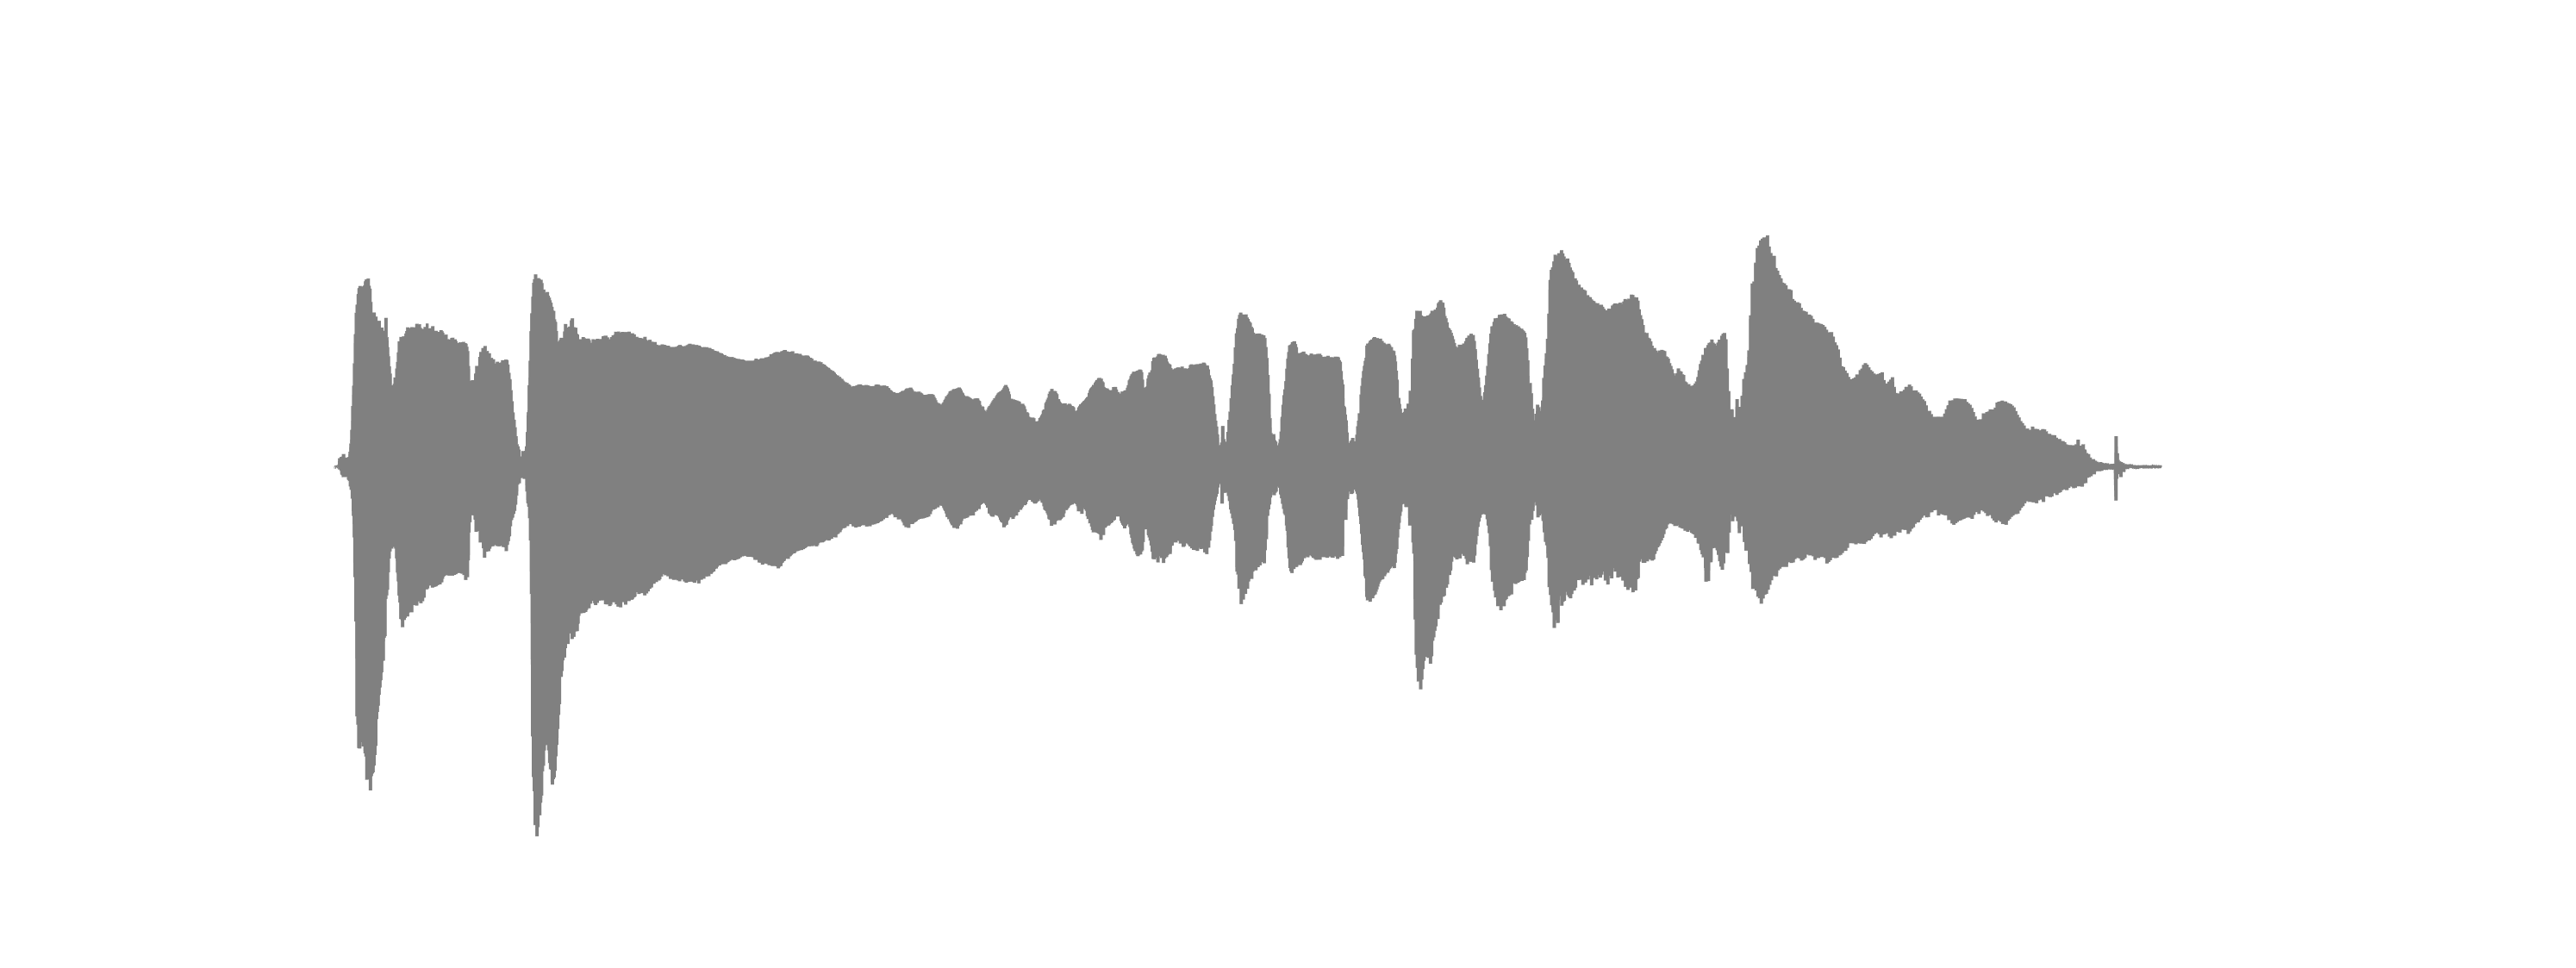
\includegraphics[scale=.2]{waveform}
            \end{textblock*}
            \begin{figure}
                \centering
\begin{footnotesize}
				\begin{picture}(96,26)
					\setcounter{iXOffset}{0}
					\setcounter{iYOffset}{5}
					\setcounter{iXBlockSize}{28}
					\setcounter{iYBlockSize}{16}
					\setcounter{iYBlockSizeDiv2}{8}
					\setcounter{iDistance}{8}
	
					\addtocounter{iYOffset}{\value{iYBlockSizeDiv2}}
					\addtocounter{iYOffset}{-2}
	
					%\addtocounter{iXOffset}{-1}
					\put(\value{iXOffset}, \value{iYOffset})
						{\text{{\shortstack[c]{audio\\ signal}}}}
					\addtocounter{iXOffset}{1}
	
					\addtocounter{iYOffset}{2}
					\addtocounter{iXOffset}{\value{iDistance}}
	
					\put(\value{iXOffset}, \value{iYOffset})
						{\vector(1,0){\value{iDistance}}}
	
					\addtocounter{iXOffset}{\value{iDistance}}
					\addtocounter{iYOffset}{-\value{iYBlockSizeDiv2}}
					
					\put(\value{iXOffset}, \value{iYOffset})
						{\framebox(\value{iXBlockSize}, \value{iYBlockSize}) {\shortstack[c]{feature extraction}}}
	
					\addtocounter{iXOffset}{\value{iXBlockSize}}
					\addtocounter{iYOffset}{\value{iYBlockSizeDiv2}}
	
					\put(\value{iXOffset}, \value{iYOffset})
						{\vector(1,0){\value{iDistance}}}
	
					\addtocounter{iXOffset}{\value{iDistance}}
					\addtocounter{iYOffset}{-\value{iYBlockSizeDiv2}}
	
					\put(\value{iXOffset}, \value{iYOffset})
						{\framebox(\value{iXBlockSize}, \value{iYBlockSize}) {\shortstack[c]{classification,\\ inference}}}
	
					\addtocounter{iXOffset}{\value{iXBlockSize}}
					\addtocounter{iYOffset}{\value{iYBlockSizeDiv2}}
	
					\put(\value{iXOffset}, \value{iYOffset})
						{\vector(1,0){\value{iDistance}}}
	
					\addtocounter{iXOffset}{\value{iDistance}}
					\addtocounter{iYOffset}{-2}
	
					\addtocounter{iXOffset}{1}
					\put(\value{iXOffset}, \value{iYOffset})
						{\text{{\shortstack[c]{class\\ labels}}}}
					
				\end{picture}
\end{footnotesize}
            \end{figure}
            
            \vspace{-3mm}
            \begin{columns}
                \column{.5\textwidth}
                    \begin{itemize}
                        \item<2->[]	\textbf{feature} representation
                                \begin{itemize}
                                    \item 	compact and non-redundant
                                    \item	task-relevant
                                    \item   easy to analyze
                                    \item   e.g., MFCCs etc.
                                \end{itemize}
                    \end{itemize}
                \column{.5\textwidth}
                    \begin{itemize}
                        \item<3->[]	\textbf{classification}
                                \begin{itemize}
                                    \item	map or convert feature to comprehensible domain
                                    \item   e.g., Support Vector Machines etc.
                                \end{itemize}
                    \end{itemize}
            \end{columns}
            \phantom{\footfullcite{burred_hierarchical_2004}}
        \end{frame}
        
        \begin{frame}{introduction}{neural network based approaches}
            
            \begin{itemize}
                \item   no custom-designed features anymore
                \item   learn features from basic inputs (like spectrograms)
            \end{itemize}
            \begin{figure}%
                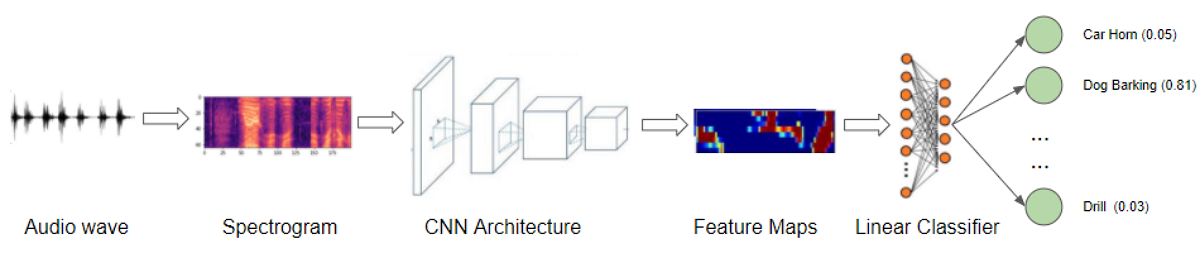
\includegraphics[width=\columnwidth]{audio_classification}%
            \end{figure}
            \pause
            \begin{itemize}
                \item   less required expert-knowledge, more complex systems
                \item   less expert-tweaking, more rigorous experimental requirement
                \item   much \textcolor{gtgold}{\textbf{higher data requirements}}
            \end{itemize}
            
            {\addreference{Fig.: \href{https://towardsdatascience.com/audio-deep-learning-made-simple-sound-classification-step-by-step-cebc936bbe5}{towardsdatascience.com/audio-deep-learning-made-simple-sound-classification-step-by-step-cebc936bbe5}}}
        \end{frame}
        
    \section{data}
        \begin{frame}{data}{importance of data}
    \vspace{-5mm}
    \begin{textblock*}{100mm}(0cm,1.5cm)
        
\includegraphics[scale=.1]{machinelearning}
    \end{textblock*}           
    
    \begin{columns}
    \column{.6\linewidth}
    \begin{itemize}
 
        \item<1->   \textbf{machine learning}: generic algorithm mapping an input to an output
            \begin{itemize}
                \item<2->   mapping function is learned from patterns and characteristics \textbf{from data}
                \item<2->[$\Rightarrow$]   model \textbf{success largely depends on training data}
                
            \end{itemize}
        \bigskip
        \item<3->   \textbf{general challenges} concerning data
            \begin{itemize}
                \item   noisiness
                \item   subjectivity
                \item   imbalance, bias, and diversity
                \item   \only<1-3>{amount}\only<4->{\textcolor{gtgold}{\textbf{amount}}}
            \end{itemize}
    \end{itemize}
    \column{.4\linewidth}
        \begin{figure}
            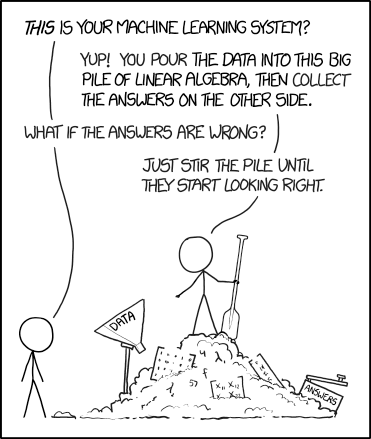
\includegraphics[scale=.4]{machine_learning}
        \end{figure}
    \end{columns}
    \addreference{\href{https://imgs.xkcd.com/comics/machine\_learning.png}{https://imgs.xkcd.com/comics/machine\_learning.png}}
\end{frame}

\begin{frame}{data}{insufficient data}
    \question{insufficient data in music}
    
    \bigskip
    \begin{columns}
    \column{.6\linewidth}
    \begin{itemize}
        \item<1->   \textbf{music data} itself is not scarce (although there might be copyright issues...)
        \smallskip
        \item<2->   \textbf{consumer annotations} are more difficult to collect, but there are some large collections
        \smallskip
        \item<3->   \textbf{detailed musical annotations} are hard to come by, because
        \begin{itemize}
            \item   time consuming and tedious annotation process
            \item   experts needed for annotations
        \end{itemize}
    \end{itemize}
    \column{.4\linewidth}
    %\vspace{-2mm}
    \begin{figure}
        
\includegraphics[scale=.1]{musicdata}
    \end{figure}
    \end{columns}
\end{frame}

        
    \section{overview}        
        \begin{frame}{overview}{overview}
            \begin{enumerate}
                \item   \textbf{semi-supervised learning }
                    \begin{itemize}
                        \item   utilize unlabeled data to improve classification
                    \end{itemize}
                \bigskip
                \item   \textbf{self-supervised representation learning }
                    \begin{itemize}
                        \item   utilize pre-trained features to improve classification
                    \end{itemize}
                \bigskip
                \item   \textbf{reprogramming} 
                    \begin{itemize}
                        \item   utilize pre-trained model to improve classification
                    \end{itemize}
            \end{enumerate}
        \end{frame}

    
    \section{semi-supervised}
        \begin{frame}{semi-supervised audio classification}{introduction}
\begin{itemize}
    \item   \textbf{observation}:
        \begin{itemize}
            \item unlabeled data is readily available 
                \begin{itemize}
                    \item example: OpenMIC dataset (musical instrument classification)
                        \begin{figure}%
                            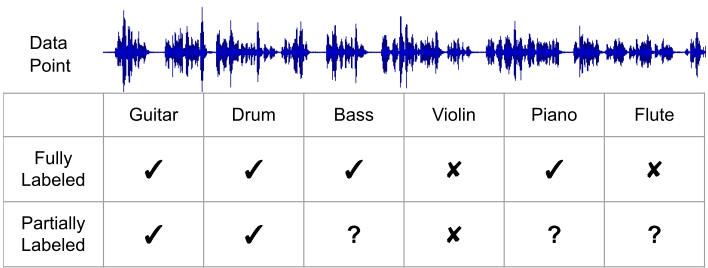
\includegraphics[scale=.3]{openmic}%
                        \end{figure}
                \end{itemize}
        \end{itemize}
    \bigskip
    \item<2->  \textbf{goal}: 
        \begin{itemize}
            \item utilize \textit{unlabeled} data for training to improve inference
        \end{itemize}
\end{itemize}
\end{frame}

\begin{frame}{semi-supervised audio classification}{experimental setup: data}
    \begin{columns}
        \column{.6\linewidth}
            \begin{itemize}
                \item   OpenMic:
                    \begin{itemize}
                        \item   20 classes of musical instruments
                        \item   \unit[10]{s} audio snippets (20000)
                        \item   90\% of labels are missing
                    \end{itemize}
                \bigskip
                \item   SONYC Urban Sound Tagging:
                    \begin{itemize}
                        \item   23 classes of urban noise
                        \item   \unit[10]{s} audio snippets ($13538+4308+669$)
                        \item   6\% of labels are missing
                    \end{itemize}
            \end{itemize}
        \column{.4\linewidth}
            \begin{figure}%
                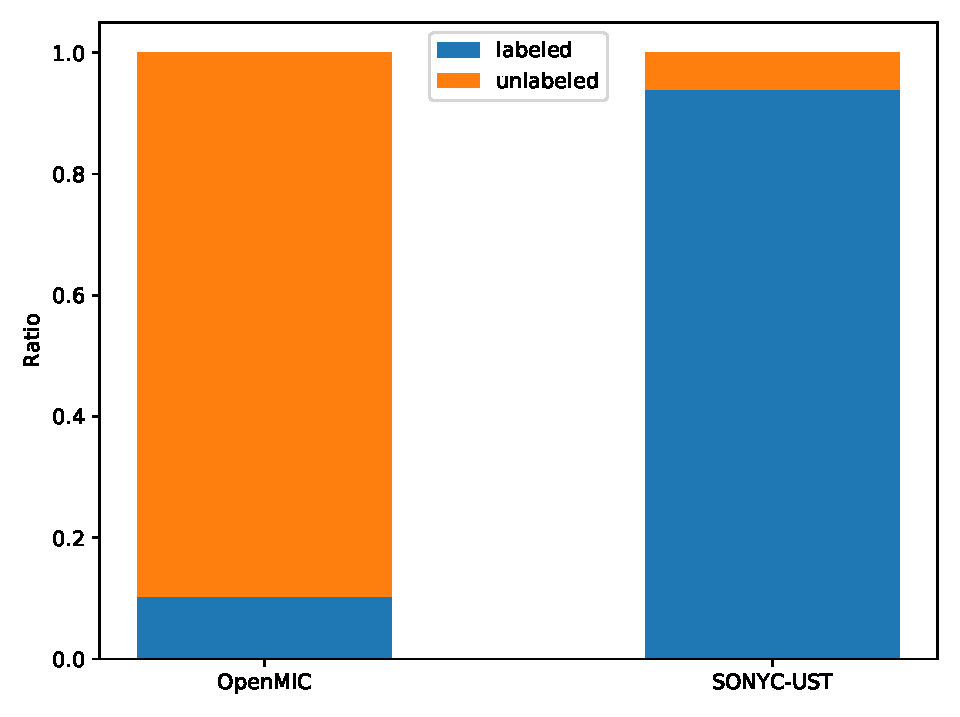
\includegraphics[scale=.3]{dataset}%
            \end{figure}
    \end{columns}
\end{frame}

\begin{frame}{semi-supervised audio classification}{experimental setup: baselines}
    \begin{itemize}
        \item Baseline 0 (B0):
            \begin{itemize}
                \item   missing labels are treated as negative labels
                \item   ``standard approach''
            \end{itemize}
        \bigskip
        \item   Baseline 1 (B1):
            \begin{itemize}
                \item   missing labels are masked out of the loss function
            \end{itemize}
    \end{itemize}
\end{frame}

\begin{frame}{semi-supervised audio classification}{method 1: label enhancing}
    \begin{columns}
        \column{.6\linewidth}
            \begin{itemize}
                \item   stage 1: 
                    \begin{itemize}
                        \item   assume all missing labels are negative 
                        \item train a teacher system
                    \end{itemize}
                \bigskip
                \item   stage 2: 
                    \begin{itemize}
                        \item   predict labels with teacher
                        \item   train student with combined training set/likely predicted labels
                        \item   mask the loss for unlikely negatives
                    \end{itemize}
            \end{itemize}
        \column{.4\linewidth}
            \begin{figure}%
                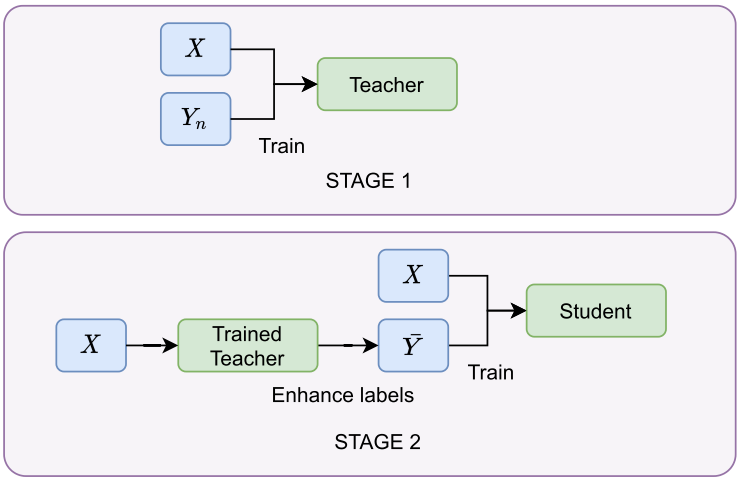
\includegraphics[scale=.3]{labelenhancing}%
            \end{figure}
    \end{columns}
    \phantom{\footfullcite{fonseca_addressing_2020}}
\end{frame}

\begin{frame}{semi-supervised audio classification}{method 2: mean teacher}
    \begin{columns}
        \column{.6\linewidth}
            \begin{itemize}
                \item   teacher and student are trained simultaneously
                \bigskip
                \item   teacher is exponential average (EMA) of student
                \bigskip
                \item   consistency loss is computed from the teacher predictions
                \bigskip
                \item   student is updated with both consistency loss and binary cross-entropy loss
            \end{itemize}
        \column{.4\linewidth}
            \begin{figure}%
                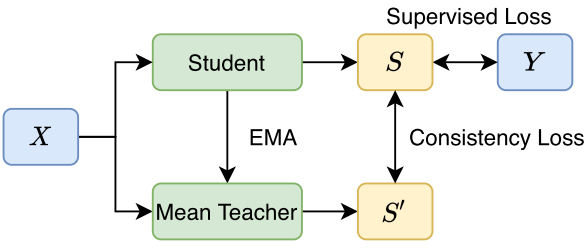
\includegraphics[scale=.3]{meanteacher}%
            \end{figure}
    \end{columns}
    \phantom{\footfullcite{bachman_learning_2014}}
\end{frame}

\begin{frame}{semi-supervised audio classification}{results: classification}
    \vspace{-5mm}
    \begin{columns}
        \column{.5\linewidth}
            \begin{itemize}
                \item   general observations
                    \begin{itemize}
                        \item B0 always worse performance
                        \item B1 much better but can be outperformed
                    \end{itemize}
                \bigskip
                \item[  (i)]   OpenMic:
                    \begin{itemize}
                        \item   Mean Teacher outperforms Label Enhancing
                    \end{itemize}
                \bigskip
                \item[(iii)]   SONYC Urban Sound Tagging:
                    \begin{itemize}
                        \item   comparable performance of Mean Teacher and Label Enhancing
                    \end{itemize}
            \end{itemize}
        \column{.5\linewidth}
            \begin{figure}%
                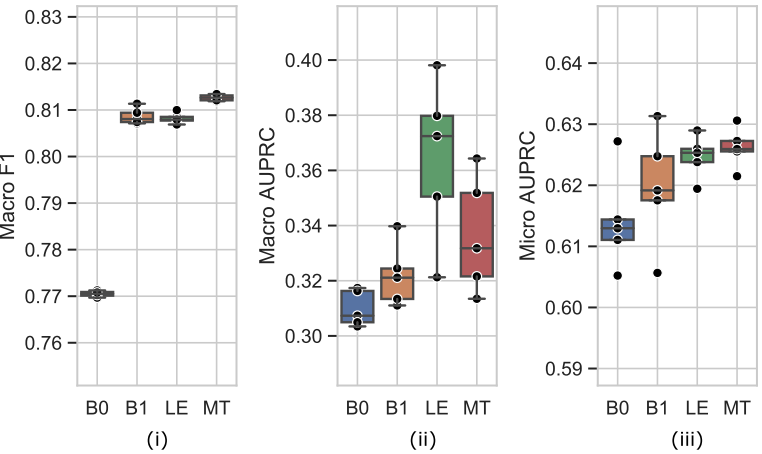
\includegraphics[scale=.3]{semi-results}%
            \end{figure}
    \end{columns}
    \phantom{\footfullcite{gururani_semi-supervised_2021}}
\end{frame}

\begin{frame}{semi-supervised audio classification}{results: data dependency}
    \begin{columns}
        \column{.5\linewidth}
            \begin{itemize}
                \item   removing labels from SONYC Urban Sound Tagging
                    \begin{itemize}
                        \item baselines deteriorate much faster
                    \end{itemize}
            \end{itemize}
        \column{.5\linewidth}
            \begin{figure}%
                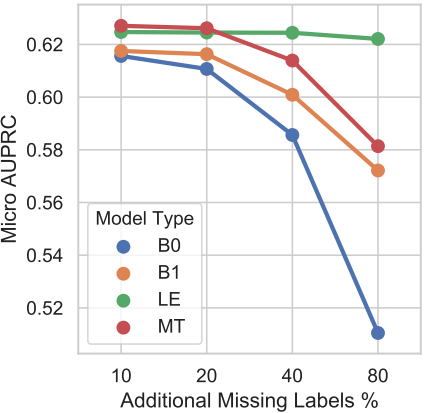
\includegraphics[scale=.45]{semi-results-data}%
            \end{figure}
    \end{columns}
    \phantom{\footfullcite{gururani_semi-supervised_2021}}
\end{frame}

    
    \section{representation}
        \begin{frame}{self-supervised representation learning}{introduction}
    \begin{itemize}
        \item   \textbf{question}:
            \begin{itemize}
                \item   how can we provide extra training information without additional data labels (related approaches: transfer learning, multi-task learning)
            \end{itemize}
        \bigskip
        \item   \textbf{idea}: 
            \begin{itemize}
                \item use proven pre-trained features (e.g., VGGish, OpenL3)
            \end{itemize}
        \bigskip
        \item<2->   \textbf{goals}:
            \begin{itemize}
                \item   \textit{impart knowledge} of pre-trained deep models (VGGish, L3)
                \item   \textit{improve model generalization} by utilizing pre-trained features
                \item   use pre-trained features \textit{only during training}
            \end{itemize}
    \end{itemize}
\end{frame}

\begin{frame}{self-supervised representation learning}{method overview}
    \begin{figure}%
        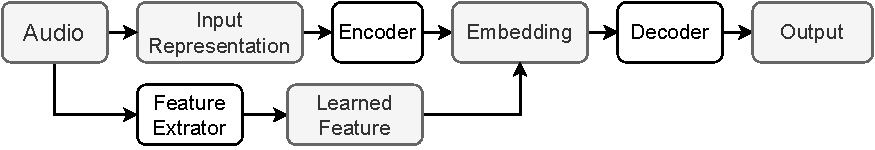
\includegraphics[width=.8\linewidth]{rep-pipeline}%
    \end{figure}
    \bigskip
    \begin{itemize}
        \item   \textbf{method 1: ``Con-Reg''}
            \begin{itemize}
                \item   make embedding space more similar to embedding space of features
            \end{itemize}
            \smallskip
        \item   \textbf{method 2: ``Dis-Reg''}
            \begin{itemize}
                \item   force distances between pairs of embedding vectors to be similar to feature distances 
            \end{itemize}
    \end{itemize}
\end{frame}

\begin{frame}{self-supervised representation learning}{experimental setup: baselines}
            \begin{itemize}
                \item   standard \textbf{transfer} learning
                    \begin{enumerate}
                        \item   extract features with pre-trained network
                        \item   train classifier for new task with feature input
                    \end{enumerate}
                    \bigskip
                \item   \textbf{concat}enation:
                    \begin{itemize}
                        \item   concatenate the pre-trained features and the learned embeddings
                        \item   classifier has the combined information (trained and pre-trained)
                    \end{itemize}
            \end{itemize}
\end{frame}

\begin{frame}{self-supervised representation learning}{experimental setup: data}
    \begin{columns}
        \column{.8\linewidth}
            \begin{itemize}
                \item   DCASE 17:
                    \begin{itemize}
                        \item   17 audio event classes
                        \item   \unit[10]{s} audio snippets ($\approx$ 53000)
                    \end{itemize}
                \bigskip
                \item   MagnaTagATune (MTAT):
                    \begin{itemize}
                        \item   50 music tags
                        \item   \unit[30]{s} audio snippets ($\approx$ 21000)
                    \end{itemize}
            \end{itemize}
        \column{.2\linewidth}
    \end{columns}
\end{frame}

\begin{frame}{self-supervised representation learning}{results: classification metrics}
    \vspace{-3mm}
    \begin{footnotesize}
    \begin{table}[]
        \centering
        \begin{tabular}{l l | c c c c | c c c c c}
           & Methods & \multicolumn{4}{c}{DCASE 17 (F1)} & \multicolumn{4}{c}{MTAT (PR-AUC)}\\
           \hline
           
           & & None & VGGish & OpenL3 & Combined & None & VGGish & OpenL3 & Combined \\
           \hline
           
           \multirow{4}{*}{BL} & Won et al.  &  0.547 & - & - & - & 0.465 & - & - & - \\
           
           & transfer & - & 0.496	& 0.477	& 0.501 & - & 0.454 & 0.454	& 0.456 \\
           
           & concat & - & 0.529 & 0.492 & 0.495 & - & 0.457 & 0.464 &	0.458\\
           
           %\midrule
           \hline
           
           \multirow{2}{*}{Prop.} & Con-Reg  & - & \underline{\textbf{0.568}} & \underline{\textbf{0.557}} & \underline{\textbf{0.576}} & - & \underline{\textbf{0.471}} & \underline{0.466} & \underline{\textbf{0.469}} \\
           
           & Dis-Reg & - & \underline{0.548} & 0.543 & \underline{0.563} & - & 0.464 & \underline{\textbf{0.468}} & 0.463 \\
          
        \end{tabular}
    \end{table}
    \end{footnotesize}
    
    \bigskip
    \begin{itemize}
        \item   two baselines \textit{cannot outperform} the trained system without additional features
        \smallskip
        \item   \textit{combining VGGish and L3 generally improves} on the individual feature results
        \smallskip
        \item   \textit{approach improves embedding space} by using pre-trained features during training
    \end{itemize}
    \phantom{\footfullcite{hung_feature-informed_2022}}
\end{frame}

\begin{frame}{self-supervised representation learning}{results: data dependency}
    \begin{itemize}
        \item   Con-Reg outperforms non-regularized system in all cases
        \item   larger improvement for lower amounts of data
    \end{itemize}
    \begin{figure}%
        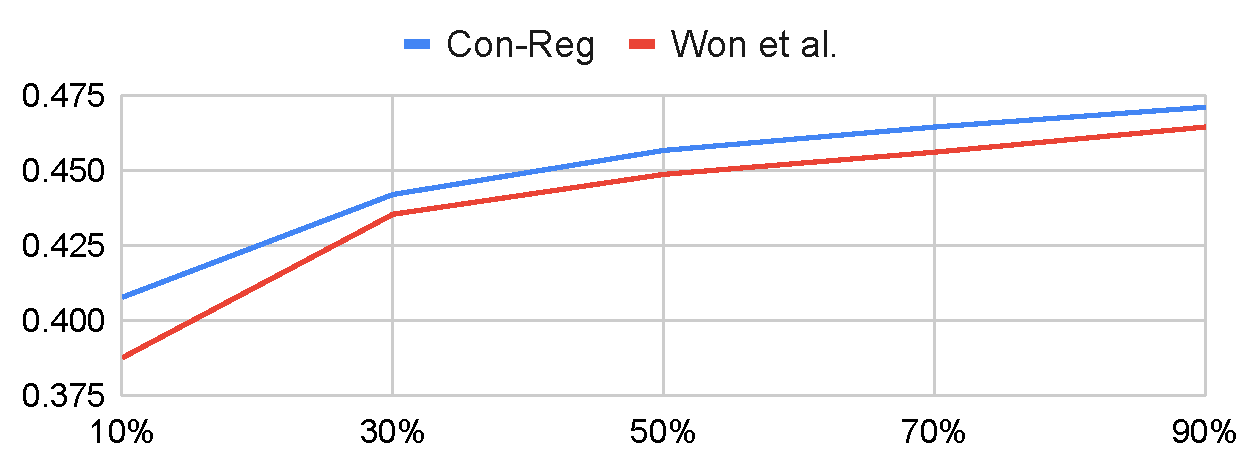
\includegraphics[scale=.45]{rep-results-data}
    \end{figure}
    
    \phantom{\footfullcite{hung_feature-informed_2022}}
\end{frame}
 
    
    \section{reprogramming}
         \begin{frame}{reprogramming}{introduction}
    \begin{itemize}
        \item   \textbf{observation}
            \begin{itemize}
                \item   pre-trained deep models can be very powerful if trained with sufficient data, even for different tasks
            \end{itemize}
        \bigskip
        \item   \textbf{idea}
            \begin{itemize}
                \item re-using pre-trained models for a new task \textbf{without} re-training
            \end{itemize}
        \bigskip
        \item<2->   \textbf{goals}
            \begin{itemize}
                \item   keep number of training parameters minimal
                \item   utilize unmodified network trained on different task
            \end{itemize}
    \end{itemize}
\end{frame}

\begin{frame}{reprogramming}{overview}
    \begin{itemize}
        \item   inspired by
            \begin{itemize}
                \item   transfer learning
                \item   adversarial learning
            \end{itemize}
        \item   allows for small trainable model (input and output processing)
    \end{itemize}
    \vspace{-2mm}
    \begin{figure}%
        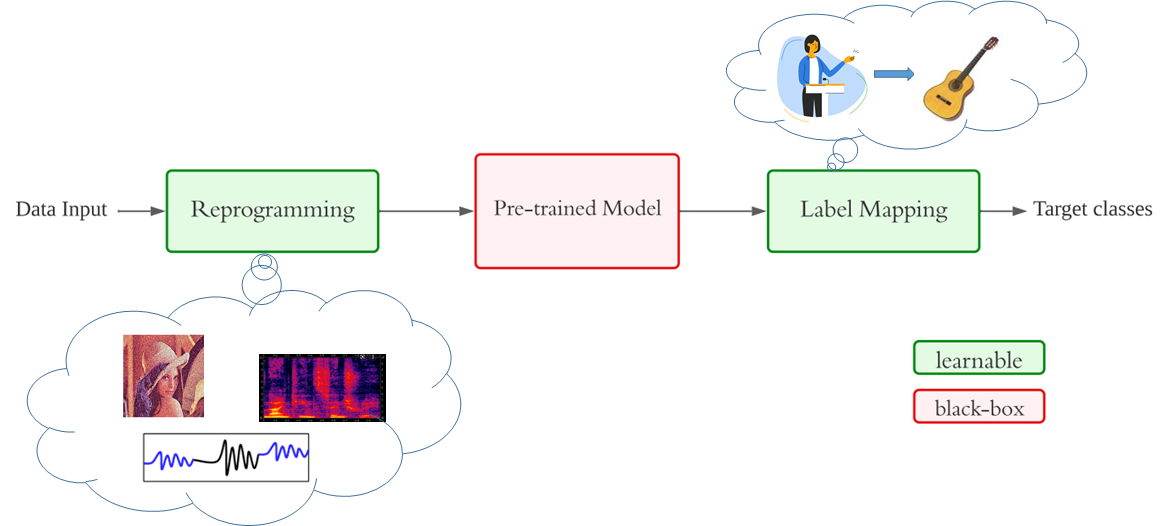
\includegraphics[width=.8\linewidth]{reprogramming}%
    \end{figure}
\end{frame}

\begin{frame}{reprogramming}{experimental setup: data}
    \begin{columns}
        \column{.8\linewidth}
            \begin{itemize}
                \item   OpenMic:
                    \begin{itemize}
                        \item   20 classes of musical instruments
                        \item   \unit[10]{s} audio snippets (20000)
                    \end{itemize}
            \end{itemize}
        \column{.2\linewidth}
    \end{columns}
\end{frame}

\begin{frame}{reprogramming}{experimental setup: baselines}
    \begin{itemize}
        \item Baseline AST:
            \begin{itemize}
                \item   state of the art performance on audio event classification\footfullcite{gong_ast_2021}
            \end{itemize}
        \bigskip
        \item   ablation study:
            \begin{itemize}
                \item   CNN only
                \item   U-Net only
                \item   CNN + AST + FC
                \item   U-Net + AST + FC
            \end{itemize}
    \end{itemize}
\end{frame}

\begin{frame}{reprogramming}{results: classification metrics}
    \begin{columns}
    \column{.7\linewidth}    
    \begin{footnotesize}
    \begin{table}[]
        \centering
        \begin{tabular}{l | c | c c c c c c c c c}
           method & F1 (macro) & train. param. (M) \\
           \hline
            AST + simple output mapping & 62.03 & 0.001\\
            CNN & 60.77 & 0.017\\
            U-Net & 62.73 & 0.017\\
            CNN + AST + FC & 78.08 & 0.017\\
            U-Net + AST + FC & \textbf{81.60} & 0.018
           
        \end{tabular}
    \end{table}
    \end{footnotesize}
    \column{.3\linewidth}
    \begin{figure}%
    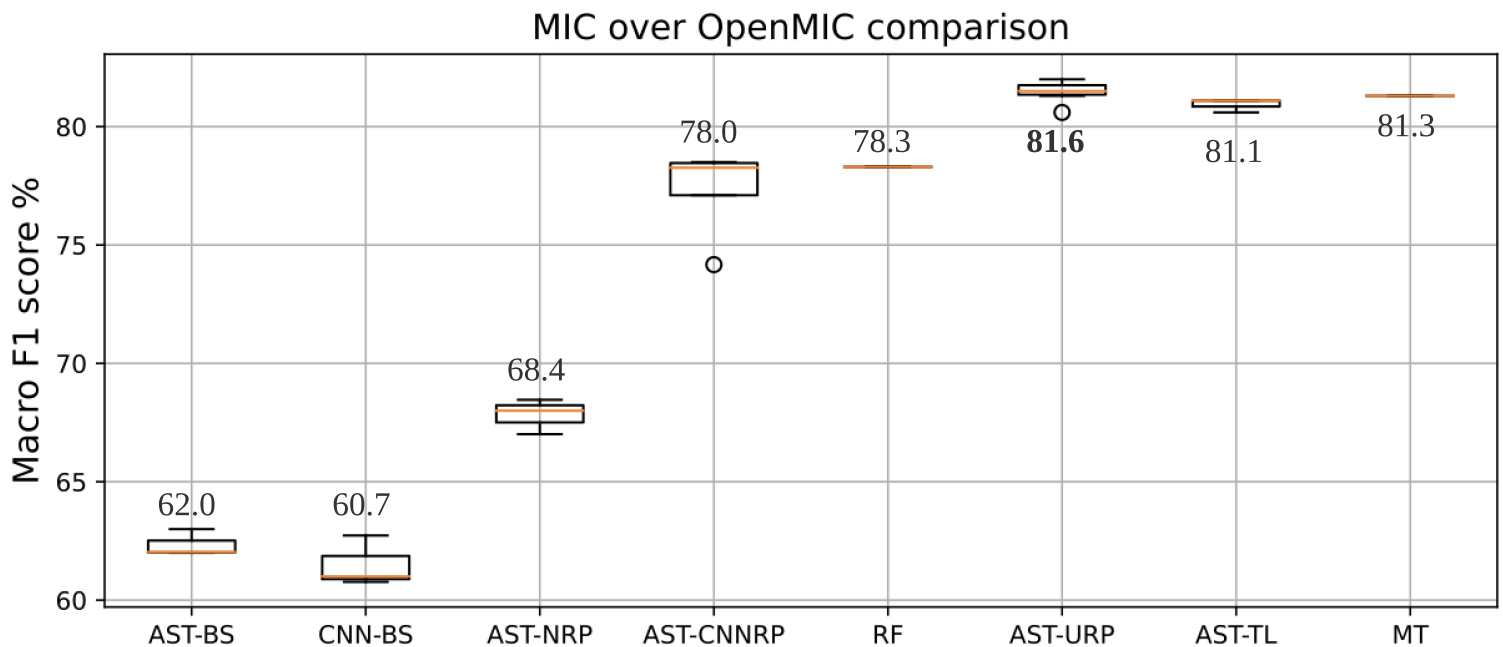
\includegraphics[width=\columnwidth]{reprog-results}%
    \end{figure}
    \end{columns}
    
    \begin{itemize}
        \item   a powerful model trained on a different task cannot easily be used directly
        \item   proper input and output processing can significantly improve performance
        \item   \textit{re-programming can beat the state-of-the-art} with a fraction of trainable parameters (at least factor 10)
    \end{itemize}
    \phantom{\footfullcite{chen_music_2023}}
\end{frame}



    \section{conclusion}
        \begin{frame}{conclusion}{learning with insufficient data}
    \vspace{-2mm}
    \begin{itemize}
        \item   literature presents many ways of \textbf{dealing with insufficient data}
            \begin{itemize}
                \item   data augmentation
                \item   data synthesis
                \item   transfer learning
                \item   semi- and self-supervised approaches
                \item   \ldots
            \end{itemize}
            \bigskip
        \item   we presented \textbf{3 recent approaches}
            \begin{itemize}
                \item   state-of-the-art \textit{semi-supervised learning}
                \item   a novel \textit{self-supervised regularization loss}
                \item   \textit{reprogramming} for audio classification
            \end{itemize}
            \bigskip
        \item   all approaches perform \textbf{at or above the state-of-the-art} with different trade-offs between
            \begin{itemize}
                \item   \textit{training complexity}
                \item   \textit{inference complexity}
                \item   \textit{classification accuracy}
            \end{itemize}
    \end{itemize}
\end{frame}

            \section[thanks]{thank you}

      \begin{frame}\frametitle{thank you!}\framesubtitle{~}
            \addreference{\href{https://github.com/alexanderlerch}{github.com/alexanderlerch}}
            \begin{block}{links}
                alexander lerch: \href{https://www.linkedin.com/in/lerch}{www.linkedin.com/in/lerch}\\             
                %\href{http://www.alexanderlerch.com}{www.alexanderlerch.com}
                
								\bigskip
								mail: \href{mailto:alexander.lerch@gatech.edu}{alexander.lerch@gatech.edu}
                
								\pause
                \bigskip                
                book: \href{https://www.AudioContentAnalysis.org}{www.AudioContentAnalysis.org}
                
                \visible<2->{
								\vspace{-25mm}
                \begin{flushright}
                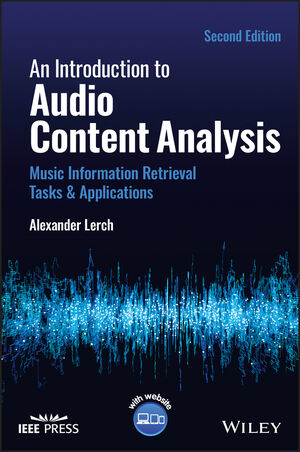
\includegraphics[scale=.20]{cover_aca2_thumb}
                \end{flushright}
                \vspace{-15mm}}

								\pause
                \bigskip
                zplane.development: 
                \href{https://www.zplane.de}{www.zplane.de}

                \pause
								\bigskip
                music informatics group:
                \href{http://musicinformatics.gatech.edu}{musicinformatics.gatech.edu}
								
								\vspace{5mm}

            \end{block}
            
			%\vspace{-22mm}
						\inserticon{mail}
            %\includegraphics[scale=.1]{wechat_qr}%
            %\begin{textblock*}{110mm}(14.25cm,7.3cm)
                %
\includegraphics[height=1.25cm,keepaspectratio]{mail}
            %\end{textblock*}            
        \end{frame}


\end{document}

